\subsubsection{QCD background in \etau channel}
\label{sec:qcdbkg}

As said at the beginning of the section, the \etau channel contains a significant QCD background that cannot be estimated with the same fake rate due to the difference in quark jet vs. gluon jet composition. The QCD background is estimated independently in the signal region, after the QCD contribution from the fake rate method is subtracted to avoid double counting, as described in the previous section.

The QCD background is estimated using a combination of the SS/OS method and an extrapolation to the final selection using a sample selected without the \MassTJ cut.

Before performing the SS/OS extrapolation, the normalization of the MC samples is checked for events selected with a same sign requirement in control regions. The \ttbar process is found to be well normalized. The W + jets and Z + jets processes are found to need correction factors of 0.86 and 1.21, respectively.
After correcting the normalization, the simulation yield in the same sign region is estimated to be $474\pm 18$ events, while the data yield is measured to be $736\pm 27$, giving $N_{\text{QCD}}^{\text{SS}}=262\pm 29$ (Fig. \ref{fig:QCDSSMET}). The QCD background before the \MassTJ cut is then $N_{\text{QCD}}^{\text{OS}} =277\pm 31$ for the LQ selection, using Eq. \eqref{bkg:QCDos}.

\begin{figure}[htbp]
  \begin{center}
    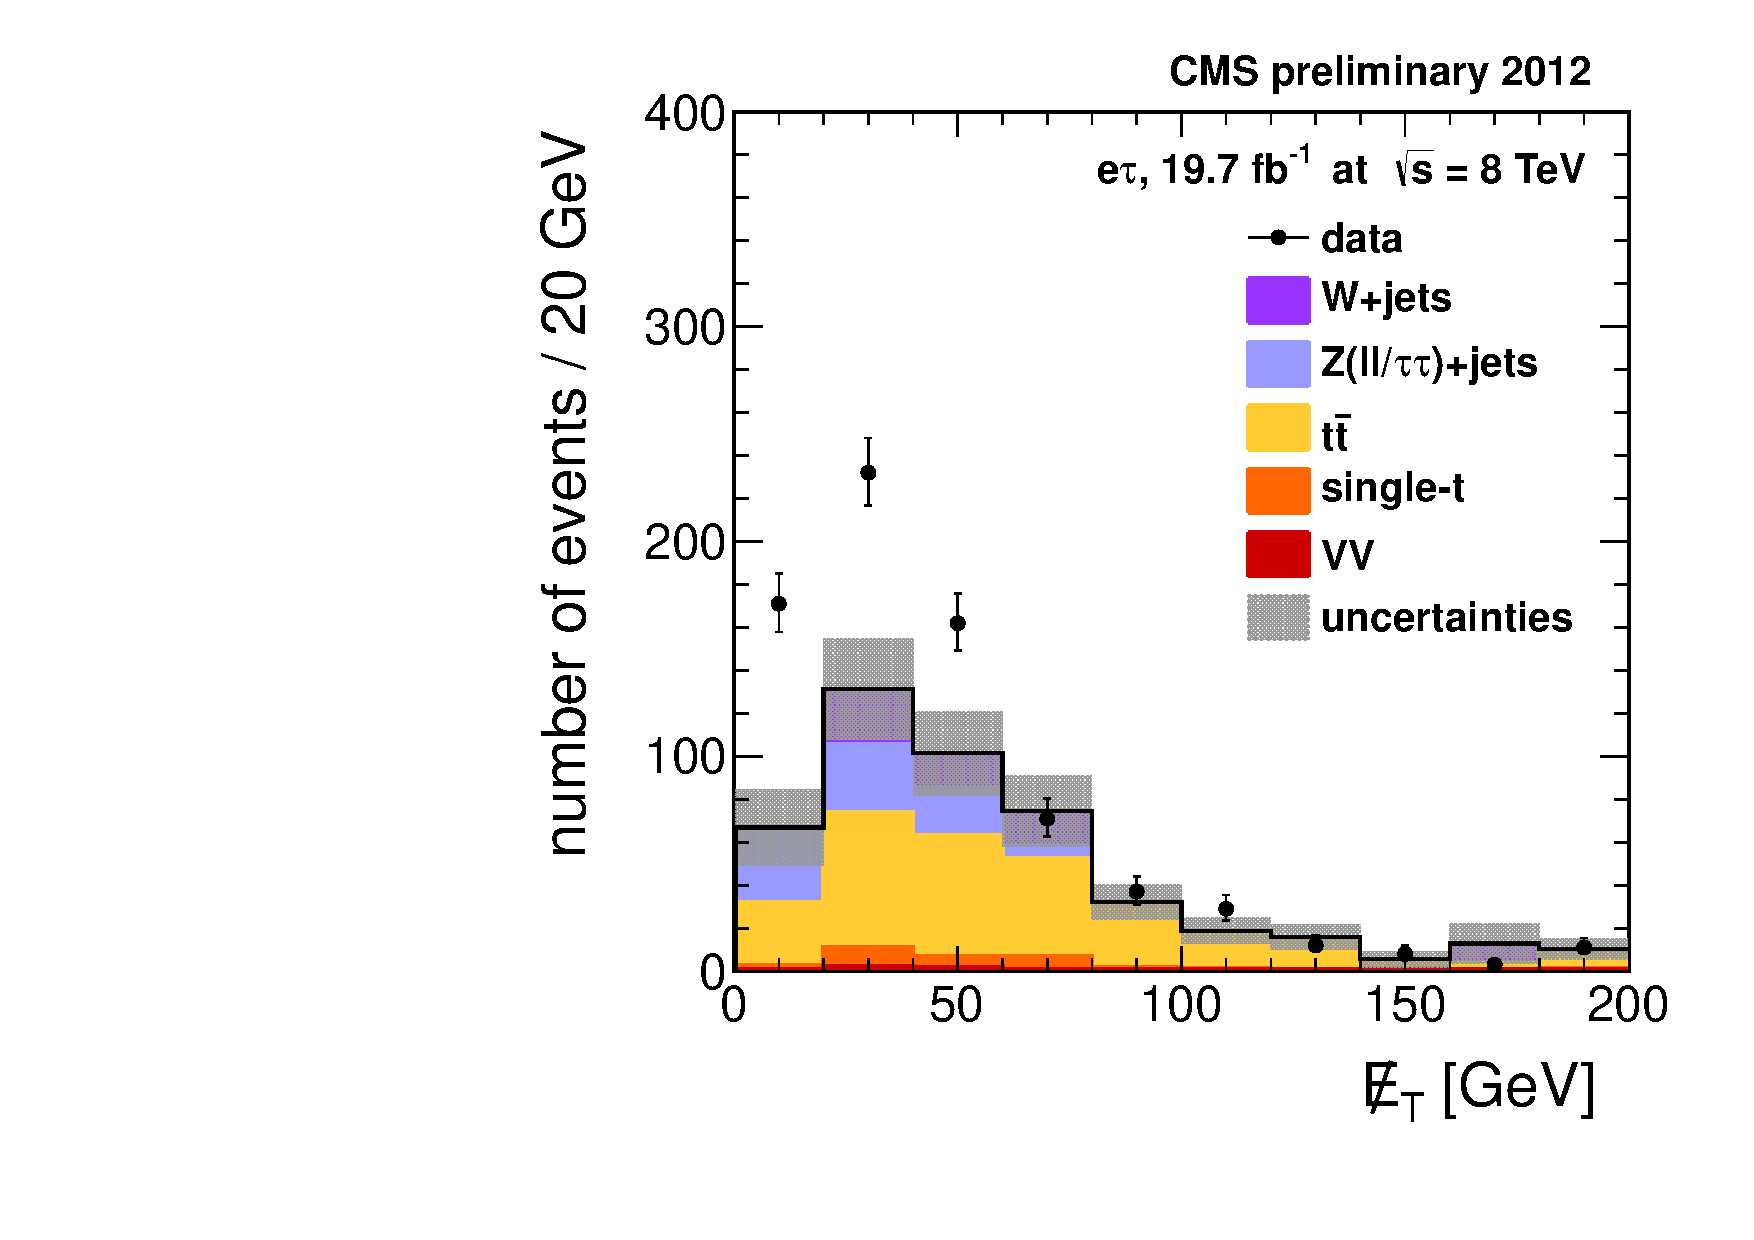
\includegraphics[width=0.6\textwidth]{figures/etau/metPtSSIso.pdf}
    \caption{Missing transverse energy spectrum for the same sign control sample, selected before the \MassTJ requirement. The excess at low \met is an indication of the presence of QCD background.}
    \label{fig:QCDSSMET}
  \end{center}
\end{figure}


The extrapolation of the QCD yield to the final selection is done by multiplying $N_{\text{QCD}}^{\text{OS}}$ by the efficiency of the \MassTJ cut on QCD events.
The efficiency is computed in a control region enriched in QCD events. This control region is selected with a same sign requirement and a veto on events containing at least one b-tagged jet. The QCD yields before and after the mass cut are defined as the subtraction of simulation from data:
\begin{eqnarray}
N_{\text{QCD}}^{\text{before}} & = & N_{\text{data}}^{\text{before}} - N_{\text{MC}}^{\text{before}} = (794\pm 28) - (469\pm 19) = 324\pm 34 \\
N_{\text{QCD}}^{\text{after}} & = & N_{\text{data}}^{\text{after}} - N_{\text{MC}}^{\text{after}} = (93\pm 10) - (66\pm 7) = 27\pm 12
\end{eqnarray}
The ratio of these two yields gives an efficiency $\varepsilon_{\text{QCD}} = 8.5\% \pm 4\%$.

Combining $N_{\text{QCD}}^{\text{OS}}$ and $\varepsilon_{\text{QCD}}$, the QCD yield after the final selection is estimated to be:
\begin{equation}
N_{\text{QCD}}^{\text{final}} = (277\pm 31) \times (8.5\% \pm 4\%) = 23.6 \pm 12 
\end{equation}
A cross check performed with the SS/OS method after the full LQ final selection gives a fully compatible, but less precise result: $N_{\text{QCD}}^{\text{SS/OS}} = 31.8 \pm 21.2$.

In addition to the yield, the QCD \ST distribution has to be defined since no MC sample is able to reproduce this shape. The shape is obtained by selecting events passing the final selection except with a same sign requirement, and subtracting the simulation from the data (Fig. \ref{fig:residQCD}). Negative values are set to zero to avoid negative entries. The obtained QCD \ST distribution is then added to the fake tau distribution obtained for the \etau channel.

\begin{figure}[htbp]
  \begin{center}
    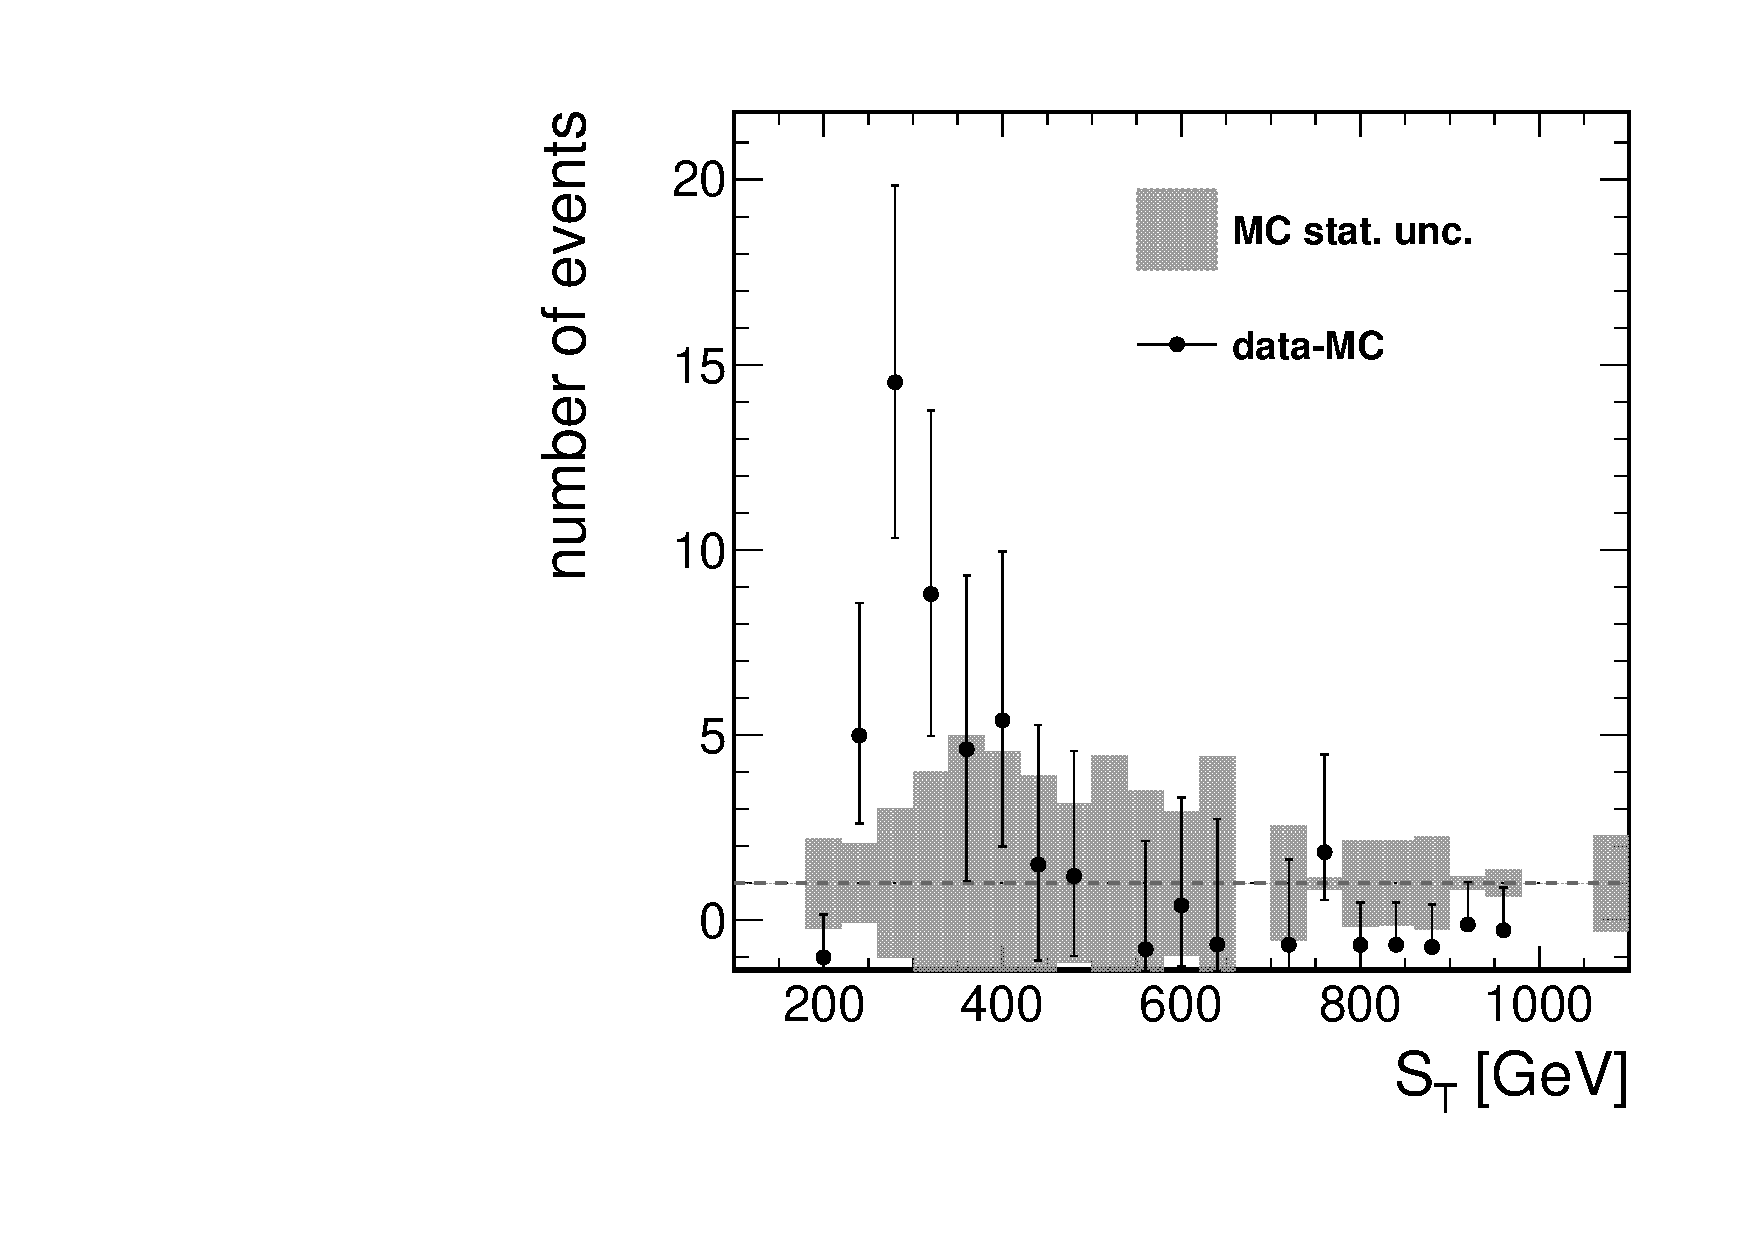
\includegraphics[width=0.6\textwidth]{figures/bkgEstim/residualQCD.pdf}
    \caption{Residual distribution (data -- simulation) for same sign events after the final selection determining the QCD shape. Negative values are set to zero before using the QCD shape.}
    \label{fig:residQCD}
  \end{center}
\end{figure}

For the LQD321 final selection, the QCD background is found to be $0 \pm 13$ using the SS/OS extrapolation method and $0 \pm 18$ using the simple SS/OS method for a cross check.
This is expected due to the high jet multiplicity requirement in this selection.






%\subsubsection{Fake tau background in \etau channel}
%\label{subsubsec:qcdbkg}

%In the \etau channel, the anti-isolated region contains a significant portion of QCD %multijet events,
%while the contribution from QCD events in the signal region is negligible.
%The fake tau objects used to calculate the fake rate are mostly quark jets, while QCD %events 
%contain mostly gluon jets. Gluon jets are wider than quark jets, so they are less %likely to 
%pass the tau isolation discriminator and therefore they have a lower fake rate. 
%Thus, applying the fake rate calculated from the \Zmm region will overestimate the 
%contribution of these QCD events to the fake tau background in the main region. 
%The QCD yield in the anti-isolated region must be estimated so that it can be %subtracted from the fake tau background estimation.

%The sample selected with isolated taus at the preselection level, before the jet %multiplicity cut, 
%is used to determine normalization corrections for \Zll, \Ztt, and W + jets MC %samples. 
%The distribution of the transverse mass of the electron and $\MET$ system, %$\MT(e,\MET)$, 
%is hypothesized to be similar for \Zll and QCD events in a W based %selection~\cite{AN-10-359,CMS:2011aa}. 
%Three normalization parameters are varied in order to minimize the difference between %the data and MC distributions of $\MT$: 

%\begin{equation}
%\MT^{(\text{data})} = r_{W}\MT^{(\text{W + jets})} + r_{\tau}\MT^{(\text{\Ztt})} + %r_{\ell}\MT^{(\text{\Zll})} + \MT^{(\text{\ttbar,single top, VV})}
%\label{Bkg:eq:MTmin}
%\end{equation}
%where $\MT^{X}$ is the $\MT$ shape for a given process $X$ (simulation on right side) %and $r_{W}$, $r_{\tau}$, $r_{\ell}$ are the three normalization parameters.

%Once the parameters $r$ are found, corrected yields are defined and used to estimate %the yield of QCD events in data.
%\begin{align}
%N(\text{W+jets}) &= r_{W}N_{\text{MC}}(\text{W+jets}) \\
%N(\Ztt) &= r_{\tau}N_{\text{MC}}(\text{\Ztt}) \\
%N(\Zll) + N(\text{QCD}) &= r_{\ell}N_{\text{MC}}(\text{\Zll}) \label{Bkg:eq:NZllQCD}
%\end{align}

%Equation \eqref{Bkg:eq:NZllQCD} follows from the hypothesis that the $\MT$ %distribution is similar in \Zll and QCD events. QCD events are not included in MC, so %the minimization in Eq.~\eqref{Bkg:eq:MTmin} scales the \Zll yield to include the QCD %yield. To solve for $N(\text{QCD})$ in terms of known quantities, it is assumed that %the corrected yield $N(\Zll)$ should be calculated using the same normalization %parameter as the corrected yield for $N(\Ztt)$.

%\begin{align}
%N(\Zll) &= r_{\tau}N_{\text{MC}}(\text{\Zll}) \\
%N(\text{QCD}) &= r_{\ell}N_{\text{MC}}(\text{\Zll}) - %r_{\tau}N_{\text{MC}}(\text{\Zll})
%\end{align}

%This method results in the following values: $r_{W} = 0.86$, $r_{\tau} = 1.21$, $r_{\ell} = 2.02$, and $N(\text{QCD}) = 24765 \pm 1411$, which is consistent with a same sign opposite sign (SS/OS) QCD estimation ($N=26424\pm1250$).
%A separate control region requiring 2 b-tagged jets and $\MT>70\GeV$ is used to find normalization factors for the \ttbar MC sample. The control region is divided into two subregions corresponding to the main region, containing isolated taus, and the anti-isolated region, containing only taus which fail isolation. The \ttbar normalization factors are found to be 0.992 for the main control region and 1.02 for the anti-isolated control region, which are close enough to 1 to be neglected. Another separate control region with $\MT>70\GeV$, $\MET>50\GeV$, and only anti-isolated taus is used to find a normalization factor of 0.96 for the anti-isolated W + jets MC sample. The Z + jets normalization factor of 1.21 is assumed to be appropriate everywhere. The corresponding normalization factors in the same sign regions are found to be very similar to the factors in the opposite sign regions.

%After finding corrected MC normalization factors, the magnitude of QCD events in the anti-isolated region is estimated using 
%the SS/OS method. A control region is defined in which the electron and tau have the same charge instead of the usual 
%opposite charge. 
%The yield of QCD events in this same sign control region is found by subtracting the MC yield from the data yield, with MC 
%normalization factors applied. The same sign QCD yield is propagated to the opposite sign region by multiplying by a 
%standard factor of 1.06~\cite{AN-13-178}. This method predicts in the anti-isolated region 
%$3026 \pm 210$ QCD events for the LQ selection and $152 \pm 15$ events for the LQD selection.

%A residual tau \pt distribution is computed by subtracting MC from data in the anti-isolated region. The fake rate is applied to this distribution in Eq. \eqref{Bkg:eq:NfakeQCD} to calculate the QCD contribution to the fake tau background estimation, which will be subtracted. The result for the LQ final selection is $38.5 \pm 2.7$ events. Similarly, $1.8\pm 0.1$ events have to be subtracted in the LQD selection.

%\begin{equation} N_{\mathrm{fake}~\tau}^{(\text{QCD})} = N_{\text{anti-iso}}^{(\text{QCD})} \sum_{\pt} \frac{\text{FR}(\pt)}{1-\text{FR}(\pt)} \label{Bkg:eq:NfakeQCD} \end{equation}

%After subtracting this overestimated QCD contribution from the fake tau background estimation, 
%the actual QCD contribution to the main region must be estimated. 
%Again, the SS/OS method is used, now in the main region. 
%The same sign QCD yield is found to be $13 \pm 19$ events for the LQ selection and $0 \pm 13.2$ for the LQD selection. 
%This is compatible with zero, so it is concluded that the QCD background in the main region after the final selection is negligible. 
%Table \ref{Bkg:tab:faketauresultsetau} shows the final results for the fake tau background in the \etau channel, with the overestimated QCD contribution subtracted from the yields which come from data in the anti-isolated region. 
%The systematic uncertainty is calculated using the same variations as in the \mutau channel, producing an overall 
%uncertainty of $21\%$ for the LQ final selection and $19\%$ for the LQD321 final selection.

%\textcolor{red}{Yields for LQD321 selection will be double-checked in the next days.}

%\begin{table}[!ht]
%  \begin{center}
%    \begin{tabular}{|c|c|c|c|c|c|}
%      \multicolumn{6}{c}{\etau channel} \\
%      \hline
%      \multicolumn{2}{|c|}{Sources} & \multicolumn{2}{|c|}{LQ Results} & \multicolumn{2}{|c|}{LQD321 Results} \\
%      \hline
%      anti-iso    & fake rate                      & yield  & variation & yield  & variation\\
%      \hline
%      data        & data (incl.)                   & 124.2 & (central)       & 74.6 & (central) \\
%      data        & data ($N_{\text{jet}} \geq 1$) & 113.9 & 10.3            & 65.7 & 8.9   \\
%      MC          & MC (incl.)                     & 129.5 & 22.7 $\text{*}$ & 77.2 & 10.5 $\text{*}$   \\
%      residual MC & data (incl.)                   & ---   & 7.1             & ---  & 2.0      \\
%      QCD & data (incl.)                           & ---   & 2.7             & ---  & 0.1     \\
%      \hline
%      \multicolumn{2}{|c|}{final result} & \multicolumn{2}{|c|}{124.2 $\pm$ 26.1} & \multicolumn{2}{|c|}{74.6$\pm$13.9}\\
%      \multicolumn{2}{|c|}{MC prediction} & \multicolumn{2}{|c|}{106.8 $\pm$ 27.3} & \multicolumn{2}{|c|}{66.7$\pm$7.6} \\
%      \hline
 %   \end{tabular}
 %   \caption{Results of the data-driven fake tau background estimation for each final selection in the \etau channel. 
%This table shows all sources of systematic uncertainty and a comparison to the generator-level MC prediction. 
%Only statistical uncertainty is given for the MC prediction. $\text{*}$ This variation is computed by comparing the MC closure test and the MC prediction.}
%    \label{Bkg:tab:faketauresultsetau}
%  \end{center}
%\end{table}
%we need to add the LQD321 final sel numbers here
